\documentclass[12pt,letterpaper,titlepage]{article}

\usepackage{fontspec}
\defaultfontfeatures{Mapping=tex-text}
\usepackage{xunicode}
\usepackage{xltxtra}
\usepackage{amsmath}
\usepackage{pdfpages}
\usepackage{amsfonts}
\usepackage{amssymb}
\setcounter{secnumdepth}{0}
\usepackage{nameref}
\usepackage{enumitem}
\usepackage{environ}
\usepackage{pdfpages}

\setmainfont{Times New Roman}
\showboxdepth=\maxdimen
\showboxbreadth=\maxdimen


\usepackage{paracol}
\usepackage{wrapfig}
\globalcounter{table}
\globalcounter{figure}
\usepackage{graphicx}
\usepackage[left=1in,right=1in,top=1in,bottom=1in]{geometry}
\graphicspath{{img/}}

\author{Jacob Abel}
\title{	Project 1A
	\\\large ECE3544 CRN:82989
}

\setlength{\parskip}{0.25em}

\begin{document}
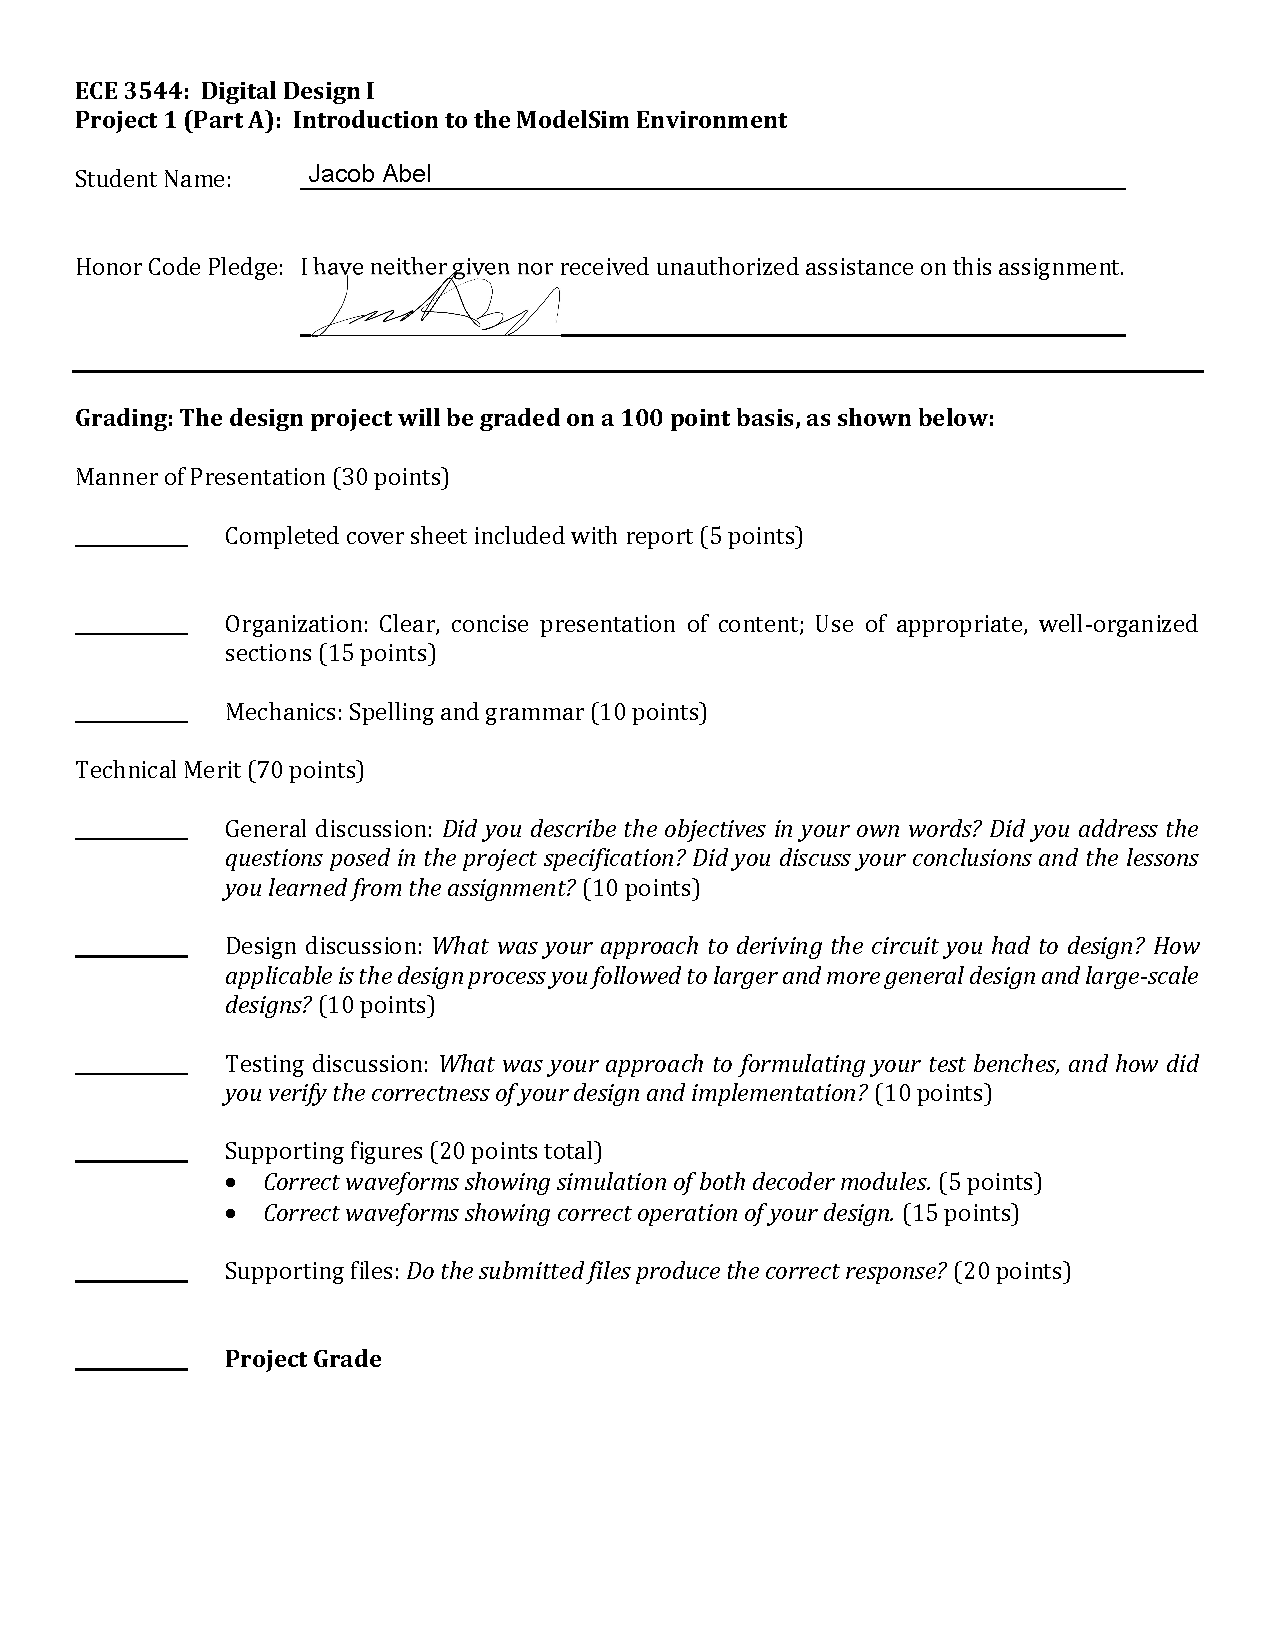
\includepdf[noautoscale]{CoverSheet.pdf}

\maketitle
\begin{raggedright}

\section*{Objective}

The objective of this project is to demonstrate basic competence with utilising ModelSim tooling and manipulating, designing, and simulating digital circuits written in Verilog.

\section{3 to 8 Decoder Gate Diagram}
\begin{center}
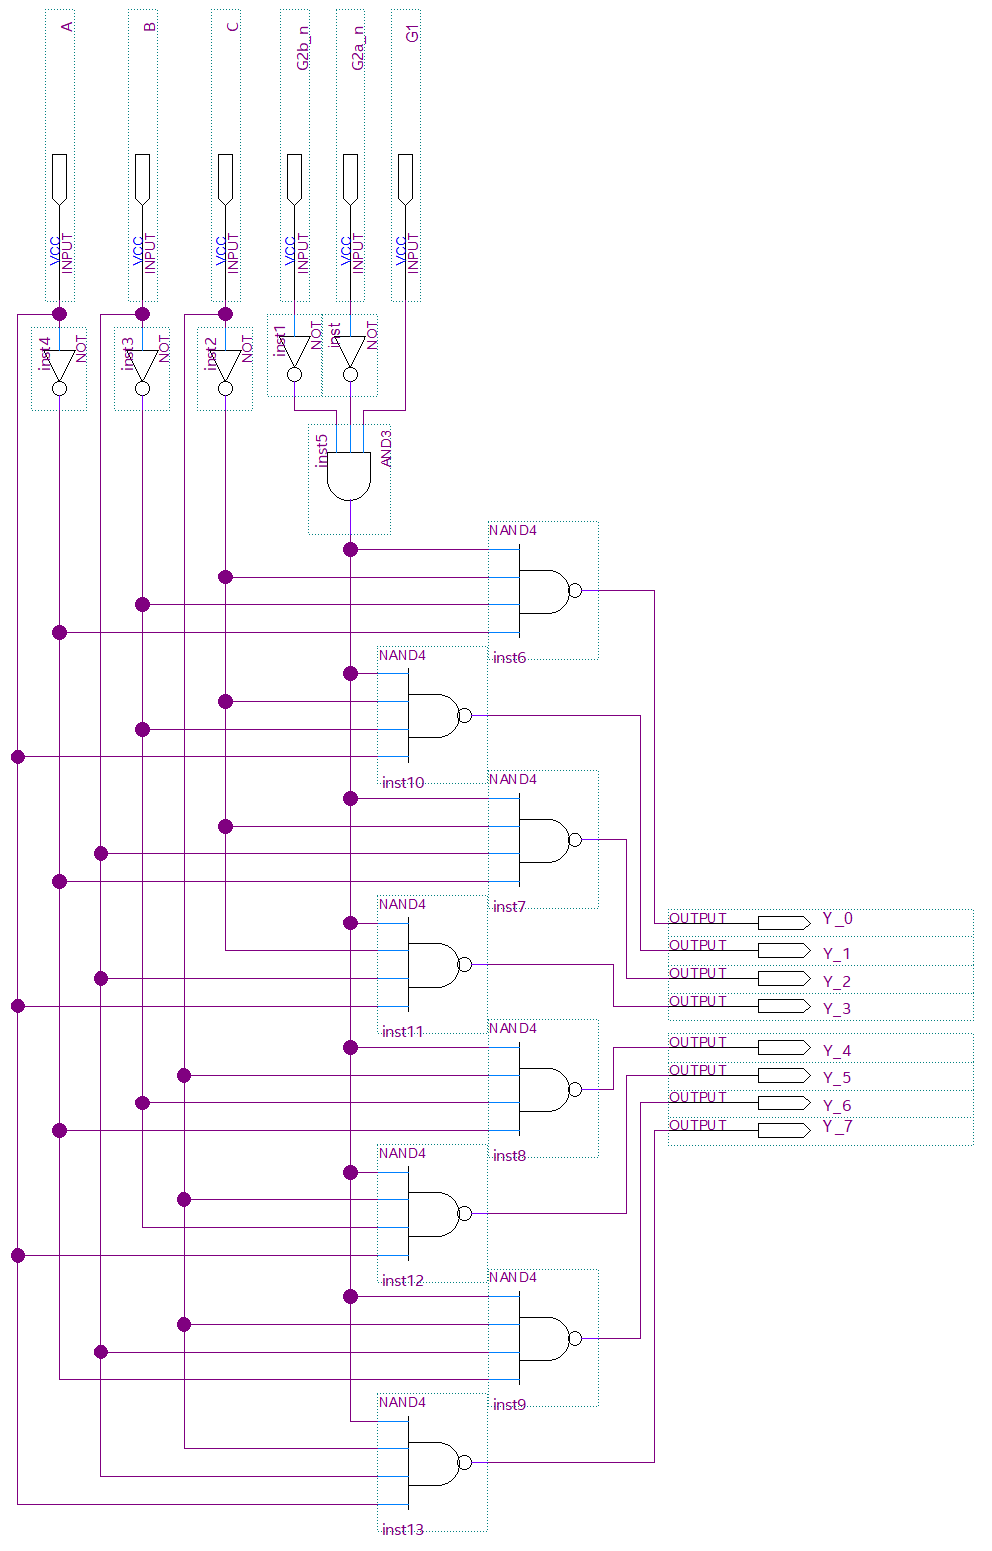
\includegraphics[width=\textwidth, height=0.8\textheight, keepaspectratio=true]{3to8}
\end{center}

\clearpage
\section{4 to 16 Decoder Block Diagram}

Note: $S_0$, $S_1$, and $S_2$ map to $A$, $B$, and $C$ respectively.
\begin{center}
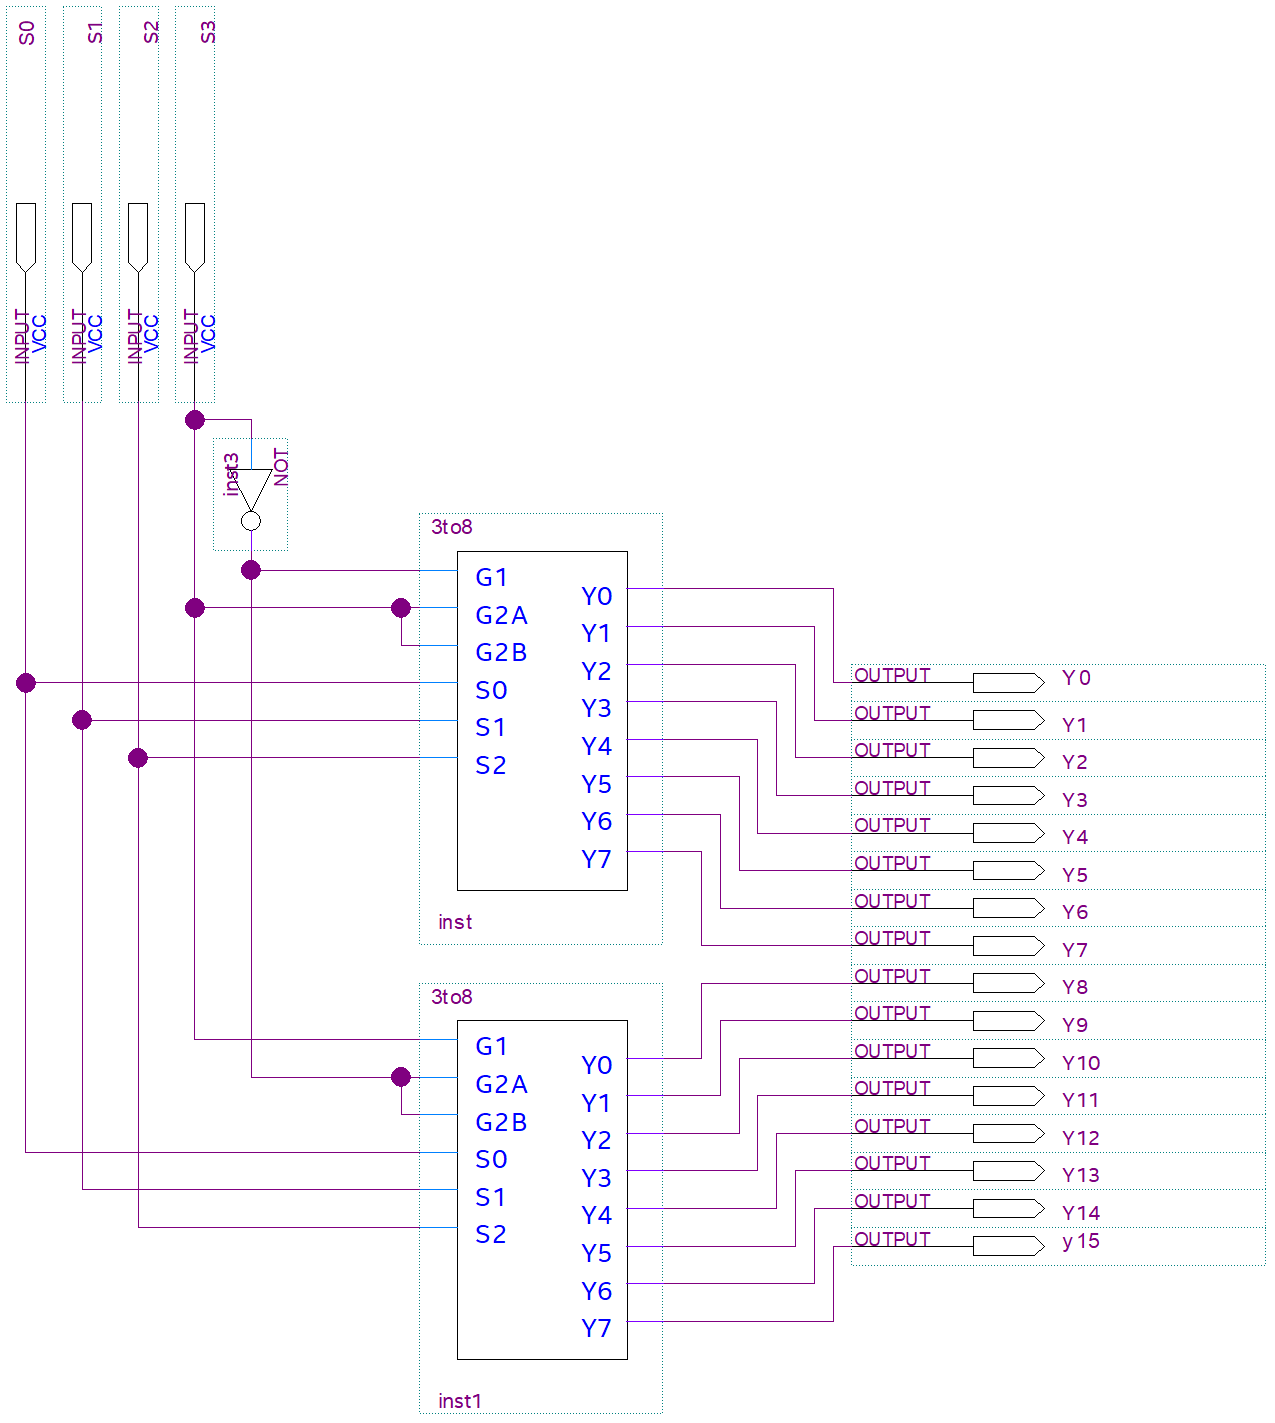
\includegraphics[width=\textwidth, height=0.6\textheight, keepaspectratio=true]{4to16}
\end{center}

\section{Test-bench Differences}

The 3-to-8 decoder and 4-to-16 decoder test-benches are fairly similar however they differ largely in the implementation of the test coverage. The 3-to-8 decoder test bench has two initial blocks which execute in parallel. This allows the possible variations of each variable to be listed together and execute all the permutations. The 4-to-16 decoder uses a for loop to loop through all possible input values.

The 3-to-8 test-bench's method is better when multiple variables have to be tested however the 4-to-16 test-bench's method is better when many inputs of one variable have to be tested. The two methods could be combined to make the 3-to-8 test-bench more concise.

\clearpage

\section{Decoder Simulation}
\begin{center}
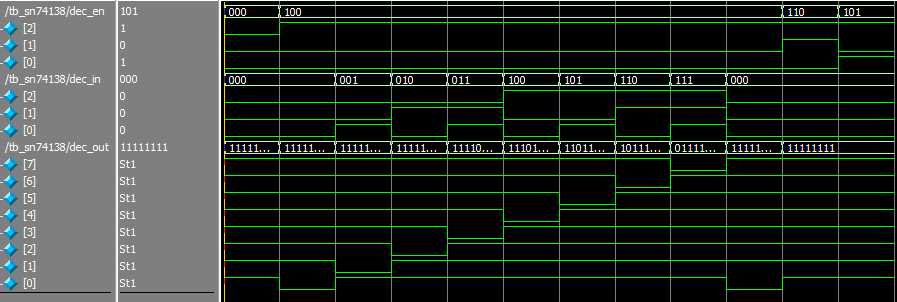
\includegraphics[width=\textwidth]{tb_3to8}
74138 3-to-8 Decoder Test-Bench Waveform
\end{center}

\begin{center}
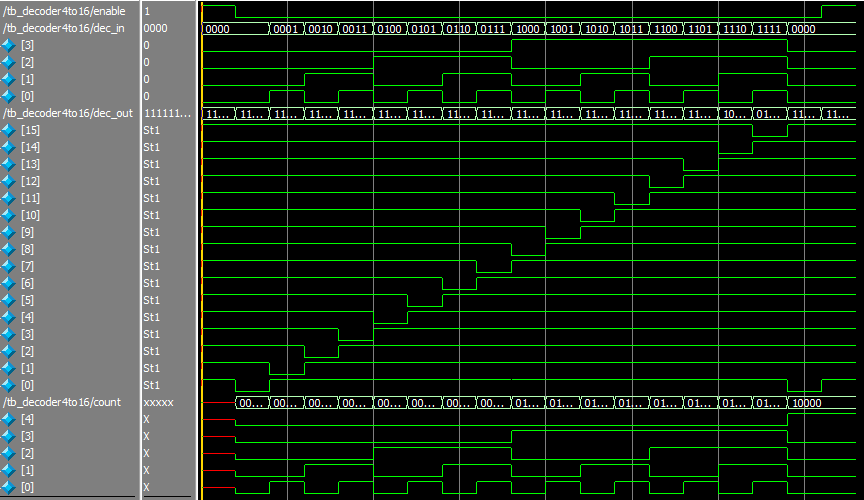
\includegraphics[width=\textwidth, height=\textheight, keepaspectratio=true]{tb_4to16}
4-to-16 Decoder Test-Bench Waveform
\end{center}

\clearpage

\section{Rock Paper Scissors Design}

The project requires that a combinatorial circuit be designed that computes the results of a "Rock, Paper, Scissors" game. The circuit accepts two inputs: \texttt{player\_a[1:0]} and \texttt{player\_b[1:0]} and outputs three 1-bit outputs: \texttt{player\_a\_wins}, \texttt{player\_b\_wins}, and \texttt{tie\_game}. The standard rules of the game apply: 
\begin{itemize}
\item Rock beats Scissors
\item Scissors beat Paper
\item Paper beats Rock
\end{itemize}

The values of the input moves are as follows.
\begin{center}
\begin{tabular}{|c|c|c|c|}
\hline 
Move & Rock & Paper & Scissors \\ 
\hline 
Input Value & 11 & 10 & 00 \\ 
\hline 
\end{tabular} 
\end{center}

\subsection*{Design Process Reflection}

The design process for this project was rudimentary however due to the simplicity of the project, it had no impact on the overall design. The design of the project was oriented primarily around rapid development and readability rather than optimisation as any optimisations that could be done at this level are trivial for a compiler.

The strategy for design was to design the system from the bottom up rather than top down. Inputs were composed into moves (Rock, Paper, Scissor) and move matchups were evaluated and grouped together by their win state (A, B, tie). The grouped matchups were or-ed together and outputted.

While this approach has some connection to large scale design, it is largely relegated to the mid and lower levels of project design as top down approaches tend to be more valuable at large scales. This methodology does however serve to compose rudimentary elements into logical blocks that can be integrated into large scale methodologies.

\clearpage
\section{Rock Paper Scissors Simulation}
\begin{center}
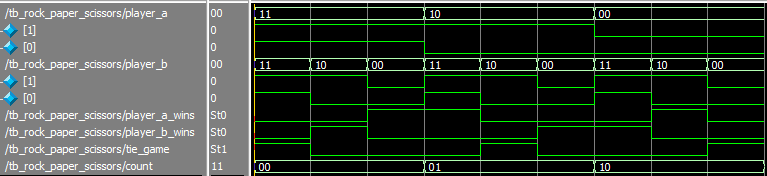
\includegraphics[width=\textwidth]{tb_rps}
Rock Paper Scissors Simulation
\end{center}

The simulation demonstrates that the code matches the intended behaviour. The test bench was designed to cover all possible inputs while minimising repetition. An initial block was used for each variable and a for loop was used for secondary variables(\texttt{player\_b}) to fill the repetitions for all states of the primary variable (\texttt{player\_a}).

\section{Conclusion}

This project served as a refresher in Verilog and an introduction to ModelSim. During this project there were a  number of issues with ModelSim configurations, mistakes with Verilog syntax, and basic logic mistakes however the project overall was a success. Unfortunately as this project was started far later than intended, many bugs came from being rushed and the project ended up taking more time and effort as a result. Luckily as this is the start of the semester, this project can serve as a reminder to start early from now on.

\end{raggedright}
\end{document}
